\documentclass[12pt,a4paper,oneside]{book}
\usepackage[spanish]{babel}
\usepackage[T1]{fontenc}
\usepackage[utf8]{inputenc}
\usepackage{fourier}
\usepackage{inconsolata}
\usepackage{marginnote}
\usepackage{texlinks}
\usepackage{adjustbox}
\usepackage{mdframed}
\usepackage{caption}
\usepackage{xspace}
\usepackage[unicode=true,pdfusetitle,
 bookmarks=true,bookmarksnumbered=false,bookmarksopen=true,
 breaklinks=false,pdfborder={0 0 0},backref=false,colorlinks=false]
 {hyperref}
\usepackage[textsize=footnotesize]{todonotes}
%\usepackage{showframe}
\usepackage{tabularx}
\usepackage{lipsum}


%% \usepackage{titlesec}
%% \titleformat{\chapter}[hang]{\Huge}{\thechapter\hspace{10pt}\textcolor{gray}{|}\hspace{10pt}}{0pt}{}
%% \titlespacing*{\chapter}{0cm}{0cm}{1cm}

\usepackage[margin=1in,marginparwidth=60pt]{geometry}

\usepackage{paralist}

\usepackage{amsmath}
\usepackage{amssymb}

\usepackage{amsthm}
\newtheorem{theorem}{THEOREM}[chapter]
\newtheorem{example}[theorem]{EXAMPLE}

\usepackage{color}
\usepackage{xcolor}

%%% Code Listings
\usepackage{listings}
\usepackage{pxfonts}
{% -*- mode: LaTeX; TeX-PDF-mode: t; TeX-master: "manual"; -*-
}

\lstset{
  basicstyle=\ttfamily,
  columns=fullflexible,
  keepspaces=true,
  commentstyle=\color{gray}\upshape
}

\lstset{language=C++}


\lstdefinestyle{script}
{mathescape=false, numbers=left, stepnumber=1, numberstyle=\tiny, numbersep=10pt, language=bash, morekeywords={esac,in}}

\lstdefinestyle{shell}
{language=bash,keywords={}}

%\adjustbox{cframe=<color> <thickness> <inner sep> <outer margin>}{<text>}
\let\lst\lstinline

\newcommand{\lt}{\symbol{"3C}}% Less than
\newcommand{\gt}{>}% Greater than
\newcommand{\xmlstructrefwb}[1]{\hyperlink{\detokenize{#1}}{\mbox{\textcolor{red}{\uppercase{\small\ttfamily\bfseries #1}}}}}
\newcommand{\xmlstructattr}[1]{{\small\ttfamily\color{orange}\bfseries #1}}
\newcommand{\xmlstructvalue}[1]{{\small\ttfamily\color{green}\bfseries #1}}
\newcommand{\xmlstructtemplate}[1]{{\small\ttfamily\bfseries\adjustbox{margin=0.4ex, bgcolor=red!20}{\detokenize{#1}}}}
\newcommand{\xmlstructdef}[2]{\hypertarget{\detokenize{#1:#2}}{\mbox{\textcolor{red}{\textbf{\textsf{\uppercase{\ttfamily\bfseries #2}}}}}}}
\newcommand{\xmlstructref}[2]{\hyperlink{\detokenize{#1:#2}}{\mbox{[\textcolor{red}{\uppercase{\small\ttfamily\bfseries #2}}]}}}
\newcommand{\xmlstruct}[3]{
\begin{mdframed}[linewidth=1pt]
\xmlstructdef{#1}{#2}\hfill

\lstinputlisting{xml/#1/#2.tex}

%\noindent
%\colorbox{yellow}{\textsc{Since Version:}} 1.0
%\medskip

\noindent
\colorbox{yellow}{\textsc{Description:}}
\medskip

\noindent
#3
\end{mdframed}
}


\newcommand{\tooldesc}[4]{
\begin{mdframed}[linewidth=1pt]

\textcolor{blue}{\textbf{\textsf{#1}}}

\bigskip
\noindent
\colorbox{yellow}{\textsc{Description:}}
\medskip

\noindent
#2

\medskip
\noindent
\colorbox{yellow}{\textsc{Further reading:}}
\medskip

\noindent
#3

\medskip
\noindent
\colorbox{yellow}{\textsc{Integration:}}
\medskip

\noindent
#4

\end{mdframed}
}

\newcommand{\abs}[0]{\textsc{ABS}\xspace}
\newcommand{\ei}[0]{\textsc{EasyInterface}\xspace}
\newcommand{\eiol}[0]{\textsc{EIOL}\xspace}
\newcommand{\eigithub}[0]{\url{http://github.com/abstools/easyinterface}\xspace}
\newcommand{\envisage}{\href{http://www.envisage-project.eu}{\textsc{Envisage}}\xspace}
\newcommand{\costa}{\href{http://costa.ls.fi.upm.es}{\textsc{Costa}}\xspace}

% web client

\newcommand{\applybutton}[0]{\begingroup\setlength{\fboxsep}{0pt}\colorbox{blue!20}{\texttt{Run}}\endgroup\xspace}
\newcommand{\refreshoutline}[0]{\begingroup\setlength{\fboxsep}{0pt}\colorbox{blue!20}{\texttt{Refresh Outline}}\endgroup\xspace}
\newcommand{\settingbutton}[0]{\begingroup\setlength{\fboxsep}{0pt}\colorbox{blue!20}{\texttt{Settings}}\endgroup\xspace}
\newcommand{\helpbutton}[0]{
\begingroup
\setlength{\fboxsep}{0pt}%  
\colorbox{blue!20}{\texttt{Help}}\xspace
\endgroup
}


% Objective
\newcounter{eiobj}
\newcommand{\objdef}[1]{%
\refstepcounter{eiobj}
{O}{\theeiobj}%
\label{obj:#1}
}

\newcommand{\objref}[1]{{O}{\ref{obj:#1}}}


\begin{document}

  \setcounter{page}{-1}


\newpage

\thispagestyle{empty}

\begin{center}

   \vspace{1cm}

   {\huge Metodolog{\'i}as {\'A}giles}\\[2ex]

   \vspace{0.5cm}

   \vspace{0.5cm}

   {\large Jes\'us Javier Dom\'enech Arellano}\\

   \vspace{0.5cm}

   MÁSTER EN INGENIERÍA INFORMÁTICA \\
   FACULTAD DE INFORMÁTICA\\
   UNIVERSIDAD COMPLUTENSE DE MADRID \\

   \vspace{0.65cm}
   \rule{2in}{0.5pt}\\
   \vspace{0.85cm}

  
\includegraphics[height=2.5in]{fig/UCM.jpg}
  
   \vspace{0.5cm}

   \vspace{0.5cm}

  Septiembre 2016\\
   \vspace{1cm}

\end{center}



%%% Local Variables:
%%% mode: latex
%%% TeX-master: "manual"
%%% End:

   \pdfbookmark[0]{Portada}{PDFPortadaPage}


\newpage
\tableofcontents
%\listoffigures
%\listoftables


\newpage
\pagenumbering{arabic}
\setcounter{page}{1}

\chapter{Introducción}
\label{ch:intro}

Este trabajo se realiza a partir de la conferencia ``Lean Software
Development'' realizada el día 4 de Abril 2016, por la ponente
Dña. Simona Puica. En ella se expuso la metodología de desarrollo del
software llamada como el título de la conferencia que es utilizada en
la empresa ``itestra''.\\

El trabajo busca ser un complemento a esa conferencia. En él se
presenta una breve historia sobre la evolución del desarrollo del
software y cómo los diferentes avances producen cambios en el
mismo. En el Capítulo~\ref{ch:tradicional} se presentan diferentes
ciclos de vida del software que son utilizados por famosas
metodologías de desarrollo y por las nuevas metodologías conocidas
como ágiles. En el Capítulo~\ref{ch:agil} se presentan dos de estas
metodologías ágiles: Scrum y Extreme Programming que hoy en día se
utilizan junto con la expuesta en la conferencia. Por último, el
Capítulo~\ref{ch:conclusiones} recoge unas breves conclusiones así
como la experiencia personal utilizando diversas metodologías y en
especial el reciente uso de la metodología Scrum en un proyecto
universitario.

\section{Historia de la Ingeniería del Software}
\label{sec:historia}

El software surge, en los años 50, como un añadido a los grandes
computadores. Las ideas iniciales eran de cierta sencillez aunque
requerían de cierta complejidad programarlas por eso se consideraba
que programar era un ``arte'' pero de los de ``andar por casa''. Este
“arte” se realizaba sin ninguna planificación previa, simplemente los
programadores trataban de hacer el programa de la mejor manera posible
realizando cambios hasta obtener el resultado deseado, este resultado
consistía en conseguir expresar algoritmos o soluciones bien conocidas
de una manera eficaz en un lenguaje de programación rudo. Cada
programa lo realiza normalmente una única persona y solía ser ella
misma el usuario final dentro de su organización, por ello los
programas se desarrollan a medida que se iban usando y si surgía un
error era el propio usuario quien lo depuraba y corregía. Por este
mismo motivo, la documentación relacionada a ese software era más bien
escasa.\\

En un segundo periodo, que puede durar hasta la mitad de los años 70,
en el que los computadores evolucionan se introducen conceptos como la
multiprogramación y los sistemas multiusuario lo que lleva a redefinir
la interacción ``hombre-máquina''. Entre otras cosas destaca la
aparición de la interactividad con la máquina en tiempo real, estas
podían recoger, analizar y transformar datos de múltiples fuentes de
manera dinámica. En este periodo ya se trata el software como un
producto y aparecen entidades especializadas en desarrollo del
software. Estas entidades establecen sus propios mecanismos de
desarrollo y planificación de software dando lugar al nacimiento de un
nuevo concepto \emph{``ingenier\'ia del software''} definida en 1972 por
F.L.Bauer como: \emph{``El establecimiento y uso de principios de ingeniería
robustos, orientados a obtener económicamente software que sea fiable
y funcione eficientemente sobre máquinas reales''}. Junto al crecimiento
del desarrollo del software crecía también el tamaño del mismo y su
complejidad, y por tanto aumentaban los errores y la dificultad de
solucionar los mismos por lo que se empezó a establecer como una
actividad necesaria el mantenimiento del software, lo cual resultaba
ser lo que más costes conllevaba.\\

Las computadoras eran capaces de realizar tareas y comunicarse con
otras computadoras compartiendo resultados y reaccionando ante
ellos. Esto nos lleva a una tercera fase en la evolución del software,
en la que comienzan los sistemas distribuidos. Comenzaron a aparecer
las redes tanto de área local como global y se buscaba un acceso
``instantáneo'' a los datos. A finales de este periodo R.Fairley define
la ingeniería del software como: \emph{``La disciplina tecnológica y de
gestión que concierne a la producción y el mantenimiento sistemático
de productos software desarrollados y modificados dentro de unos
plazos estipulados y costes estimados''}. Pero el uso de las
computadoras seguía siendo académico e industrial.\\

La aparición de los microprocesadores produce que la computadora se
extienda a los hogares para uso personal y de ocio. Incluso se
incluyen los microprocesadores en otros elementos como son los
electrodomésticos y se desarrolla software específico para estos. Esta
cuarta fase da lugar a la búsqueda de la estandarización y como
referente, el IEEE define en 1990 la ingeniería del software como:
\emph{``(1) La aplicación de un enfoque sistemático, disciplinado y
  cuantificable del desarrollo, la operación y el mantenimiento del
  software. (2) El estudio de enfoques tales como (1)''}. Esta fase
podría asemejarse al segundo periodo llevando lo industrial y
académico a lo personal y ocio. Por lo que las técnicas de desarrollo
aunque evolucionan siguen teniendo en cuenta los mismos
fundamentos. Algunas de las técnicas utilizadas en el desarrollo de
software en los
periodos dos, tres y cuatro se explican en el Capítulo~\ref{ch:tradicional}.\\

Es en el nuevo milenio cuando, con la globalización de Internet,
encontramos una revolución en el desarrollo del software. Se busca
principalmente sacar productos al mercado cuanto antes, manteniendo un
alto nivel de fiabilidad y calidad. El desarrollo se basa en
prototipos y en avances incrementales. Un software triunfa si es el
primero en realizar una funcionalidad, no hace falta que lo haga
perfecto si gana una masa de usuarios suficiente es difícil que una
aplicación que realice la misma tarea de mejor modo le quite su
mercado. Es por esto que nacen las nuevas metodologías de desarrollo
ágil, que como su nombre indica consiguen obtener resultados
rápidamente.

\chapter{Ciclos de vida del Software}
\label{ch:tradicional}

En este apartado se presentan diferentes modelos de ciclo de vida de
un software que dan lugar a diferentes metodologías de desarrollo del
mismo. Un ciclo de vida cumple las siguientes características:
\begin{itemize}
\item Describe las etapas principales de desarrollo de software.
\item Define las fases primarias esperadas de ser ejecutadas durante
  esas etapas.
\item Ayuda a administrar el progreso del desarrollo.
\item Provee un espacio de trabajo para la definición de un proceso
  detallado de desarrollo de software.
\end{itemize}
Para cada etapa definida en el modelo de ciclo de vida se deben
establecer una serie de objetivos, tareas y actividades que lo definan
y caractericen. La elección de un modelo para un proyecto es realmente
importante, por ello se han elaborado diferentes modelos que se
adapten a los posibles tipos de proyecto; el orden de las etapas del
ciclo de vida del modelo es uno de los puntos más importantes a la
hora de diferenciarlos. A continuación, se muestran algunos de estos
modelos.

\section{Modelo en Cascada}
\label{sec:cascada}

Este modelo, uno de los más antiguos (se dice que fue el primero), se
caracteriza por establecer un orden muy riguroso en la consecución de
las etapas del ciclo de vida. De esta manera cada etapa comienza al
finalizar la anterior y nunca hay superposición en el tiempo de las
etapas. Por ello, el modelo en cascada se le denomina como un proceso
de desarrollo secuencial en el cual vas avanzando hacia abajo (como
una cascada) a medida que vas superando etapas.\\
 
El modelo en cascada se considera como el primer modelo introducido y
utilizado en la ingeniería del software. A este modelo se le atribuye
el mérito de dividir el proceso que conlleva al ingeniería del
software en etapas bien separadas.\\

Cierto es que para poder utilizar este modelo los integrantes del
equipo de desarrollo deben tener mucha experiencia para poder definir
los pasos y tareas de manera proporcionada, ya que detectar un error
en una etapa avanzada conlleva volver a la primera etapa o la anterior
y realizar tareas de nuevo. Será Winston W. Royce en 1970 quien
describe por primera vez de manera formal este modelo, las etapas que
publicó pueden apreciarse en la Figura~\ref{fig:cascada}.\\

\begin{figure}[h]
\hrule\smallskip
\begin{center}
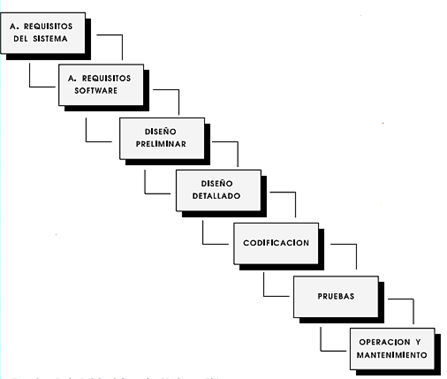
\includegraphics[width=0.8\textwidth]{fig/cascada.png}
\end{center}
\caption{Etapas del Modelo en Cascada}
\label{fig:cascada}
\hrule
\end{figure}

\paragraph{Ventajas}
Este modelo es ideal, generalmente, para proyectos grandes de carácter
estable (en especial aquellos que no tengan posibilidad de cambio en
los requisitos), es decir, proyectos donde es posible predecir de
manera completa el área del problema a resolver y así los diseñadores
puedan definir un diseño correcto y completo antes de comenzar las
fases de implementación. Por otro lado, este modelo también puede ser
utilizado en proyectos de menor envergadura donde todos los requisitos
estén bien establecidos.
 
La organización de este modelo y su diferenciación en las fases hace
que su utilización sea sencilla ya que esta rigidez produce que cada
fase tenga unos pasos bien definidos y unos entregables específicos y
un proceso de revisión de la fase, por lo que cada fase se
realiza. procesa y completa de una vez.


\paragraph{Inconvenientes}

El mayor inconveniente es que en la vida real es difícil encontrar
proyectos de ingeniería del software donde exista dicha estabilidad y
mucho menos sigan un proceso secuencial, por lo que la utilización de
este modelo resultaría una elección equivocada que conlleva al fracaso
del proyecto.
 
Otro inconveniente es que todos los resultados o mejoras que se pueden
ir haciendo no son visibles de manera progresiva, solo pueden verse
cuando el producto está terminado, esto puede provocar una inseguridad
y desconfianza por parte del cliente que siempre gusta de ir viendo
avances en el producto y opinar sobre el camino que está tomando. Esto
afecta también en el momento de tener que añadir un requisito que no
fue tomado en cuenta al comienzo del proyecto, y que surgió,
seguramente, en la etapa de la codificación. Este hecho sucede
bastante a menudo y en este modelo te obliga a volver a la etapa de
requisitos y repetir tareas ya finalizadas.

\section{Modelo de Prototipos}
\label{sec:prototipos}
El modelo basado en prototipos no determina una serie de etapas sino
que define un comportamiento en cada etapa. La construcción de
prototipos ha de comenzar desde la primera etapa del ciclo de vida del
software, es decir desde la recolección y especificación de requisitos
primera. Para llevar a cabo este modelo, es necesario que el
desarrollador y el cliente se encuentren y definan cuáles serán los
objetivos globales del software a desarrollar, así como identificar
los requisitos conocidos. A partir de esta información se debe
realizar un diseño rápido que se centre en representar esos aspectos
que serán más visible para el usuario o cliente, este diseño se
concreta en la elaboración de un prototipo. El prototipo será evaluado
y se irá refinando junto con los requisitos del software. Los avances
en las etapas permiten al cliente ver como va el proyecto y al
desarrollador comprender qué es lo que el cliente quiere que haga.

\begin{figure}[h]
\hrule\smallskip
\begin{center}
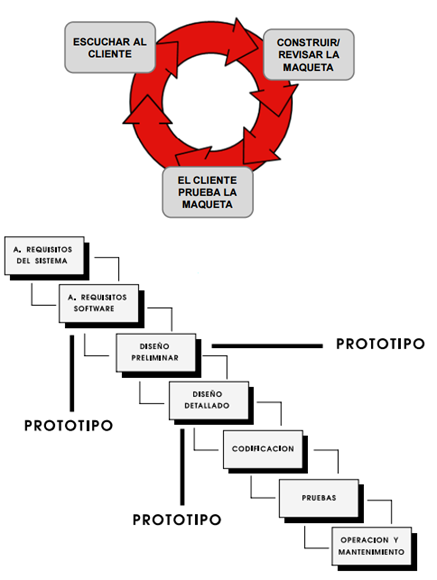
\includegraphics[width=0.5\textwidth]{fig/prototipo.png}
\end{center}
\caption{Ejemplo del Modelo de prototipos y Ciclo de trabajo.}
\label{fig:prototipos}
\hrule
\end{figure}

Se puede hacer un prototipado de diferentes maneras:
\begin{itemize}
\item Prototipado rápido:
  \begin{itemize}
  \item No modifica el ciclo de vida.
  \item Baja calidad y robustez.
  \item Evita producir cosas no solicitadas por el cliente.
  \item Reduce costes.
  \end{itemize}
\item Prototipado evolutivo:
  \begin{itemize}
  \item Funcionalidad progresiva.
  \item Construir software para que pueda ser modificado fácilmente.
  \item No se conocen niveles apropiados de calidad y documentación.
  \end{itemize}
\item Prototipado operacional:
  \begin{itemize}
  \item Mezcla rápido y evolutivo.
  \item Se basa en la siguiente imagen.
  \end{itemize}
\end{itemize}


\paragraph{Ventajas}

Este modelo de proceso tiene la gran ventaja de poder observar desde
el comienzo del ciclo de vida del software versiones posibles del
producto (los prototipos). Con ello, tal y como se ha comentado
anteriormente, el cliente puede conseguir definir mejor qué
necesidades reales tiene y cuáles son los requisitos del
producto. Esta realimentación continua del cliente nos lleva a evitar
malas sorpresas al final del proceso.

Cada prototipo puede sustituir a los documentos que indican la
situación del proyecto, aportando una realidad visual del estado del
proyecto. Además deja entrever el buen funcionamiento que tendrá el
producto final.

\paragraph{Inconvenientes}
El mayor inconveniente de este modelo es la propia realización de
prototipos que en muchos casos son productos que requieren una
inversión y que acabarán en la basura, aunque se haya aprendido
gracias a él. Si no se controla y elige bien el tipo de prototipo a
realizar puede conllevar un aumento de los costes del desarrollo del
producto.

Además, tener versiones semi-funcionales y mostrarlas al cliente
pueden llevar a una falsa ilusión del buen avance del proyecto, si no
comprende la utilidad y finalidad de los prototipos. Por último, el
desarrollador puede comprometer la calidad y el mantenimiento del
software dado que para un prototipo se puede ``cablear'' una solución
temporal que después conlleve cambios en los diseños.

\section{Modelo Incremental}
\label{sec:incremental}

Este modelo de proceso combina los dos anteriores, de modo que obtiene
la filosofía interactiva del modelo basado en prototipos y la
fiabilidad del modelo en cascada. Este modelo va incrementando la
funcionalidad del software, de modo que se aplica el modelo en cascada
con un conjunto de requisitos limitados a una o dos funcionalidades y
al terminar el producto es un prototipo, al realizar este proceso
añadiendo funcionalidades vas obteniendo diferentes prototipos hasta
que consigues el producto final.

Algunas de las principales características del modelo incremental son
las siguientes:
\begin{itemize}
\item Soluciona el problema del modelo en cascada eliminando la
  secuenciación lineal.
\item El producto final es el resultado de ir añadiendo componentes
  funcionales en forma de incrementos.
\item El software es analizado en partes de modo que no se ve como un
  producto a entregar a una fecha fija, sino como un producto
  resultado de trabajos incrementales.
\item Al ir añadiendo funcionalidades se puede adaptar a entornos
  donde hay incertidumbre en los requisitos, de modo que se van
  desarrollando funcionalidades según van apareciendo necesidades.
\end{itemize}

  

\begin{figure}[h]
\hrule\smallskip
\begin{center}
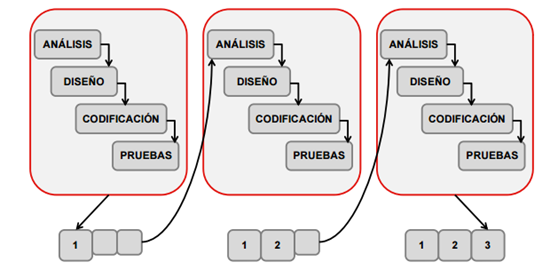
\includegraphics[width=0.8\textwidth]{fig/iterativo.png}
\end{center}
\caption{Modelo Incremental de tres fases.}
\label{fig:iterativo}
\hrule
\end{figure}

\paragraph{Ventajas} Las ventajas más importantes de este modelo corresponden con sus principales características, además aporta otras ventajas como:
\begin{itemize}
\item Reduce el coste en los cambios de alcance o requisitos del
  software.
\item Se simplifican las tareas de testing y depuración al solo tener
  que analizar una iteración pequeña cada vez.
\item Los riesgos referentes al desarrollo son más gestionables debido
  a que una iteración no contiene la totalidad del desarrollo, que
  suceda un riesgo afectaría al desarrollo de una funcionalidad y no
  al producto completo.
\item Al igual que el modelo basado en prototipos, cada iteración
  corresponde a un hito en el programa del proyecto que es fácilmente
  gestionable.
\end{itemize}


\paragraph{Inconvenientes}
Este modelo presenta varios inconvenientes, uno de ellos es la
necesidad de experiencia en el equipo para definir incrementos de modo
que no sean excesivamente pequeños ni demasiado grandes para poder
distribuir el trabajo de forma proporcionada y no realizar iteraciones
con todo su coste para un incremento insignificante. Otros
inconvenientes que aparecen al utilizar este modelo son:
\begin{itemize}
\item Cada iteración es secuencial y no es posible superponerlas entre
  sí.
\item Al no definir todos los requisitos completos al inicio pueden
  surgir incompatibilidades entre los mismos. Además, pueden dar
  problemas en la arquitectura del software, dado que en las primeras
  iteraciones se ha podido no preparar bien para integrar alguna
  funcionalidad de iteraciones posteriores.
\end{itemize}


\section{Modelo en Espiral}
\label{sec:espiral}

Barry Boehm en 1985 desarrolló el modelo en espiral, publicado en 1988
en el artículo ``A Spiral Model of Software Development and
Enhancement'', que ha sido y es utilizado de forma muy
generalizada en todo el ámbito de la ingeniería del software. El
nombre del modelo proviene de la forma en que se propone colocar las
actividades y etapas del desarrollo del software. Esta forma es una
espiral partiendo del centro, y cada vuelta corresponde a un ciclo
completo en que las actividades de ese ciclo se fijan en función de
los análisis y resultados del ciclo anterior.\\

 
Al igual que el modelo iterativo, este modelo parte de ideas básicas
del modelo basado en prototipos y el modelo en cascada. Este modelo
resulta idóneo para proyectos de larga duración, que sean caros y
complejos en su elaboración.\\

Cada ciclo de la espiral debe pasar por al menos cuatro etapas. La
primera de ellas es determinar y fijar objetivos, esto incluye
determinar los entregables, y realizar la planificación. La segunda
etapa es la encargada de hacer un análisis de riesgos estudiando
alternativas para reducirlos y eliminarlos. Como tercera etapa se
contempla todo el proceso de desarrollo, verificación y validación del
software, es la etapa de propia de creación y programación. En la
cuarta y última etapa, se revisa todo el trabajo realizado, se evalúa
y se pre-planifican las siguientes fases, y en concreto el siguiente
ciclo. Podemos observar este proceso en la Figura~\ref{fig:espiral}
comenzando en el centro y siguiendo hacia afuera en el sentido de las
agujas del reloj.

\begin{figure}[h]
\hrule\smallskip
\begin{center}
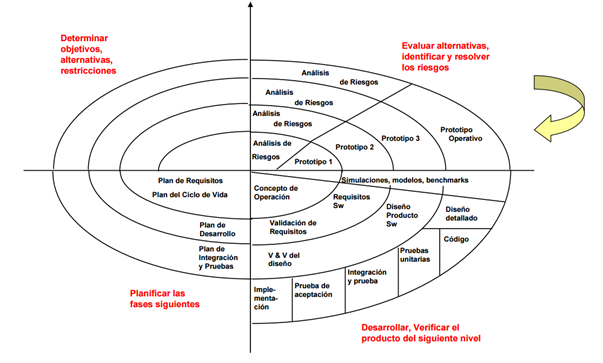
\includegraphics[width=0.7\textwidth]{fig/espiral.png}
\end{center}
\caption{Modelo en Espiral}
\label{fig:espiral}
\hrule
\end{figure}

\paragraph{Ventajas} Al realizarse el análisis de riesgos de una modo
claro y explícito se consigue reducir los riesgos del proyecto y
permite incorporar objetivos centrados en obtener calidad. Además
pueden añadirse ciclos donde se desarrolle el mantenimiento del
software. Añadir nuevos requisitos y mejoras puede hacerse sin romper
el modelo o volver a empezar, todo gracias a que el ciclo de vida no
es rígido.

\paragraph{Inconvenientes} Quizá su mayor problema es que utilizar
este modelo conlleva realizar mucho trabajo adicional, por la alta
exigencia que tiene en los análisis de riesgos. Esto conlleva a
necesitar experiencia y analistas expertos en esta tarea. Este modelo
es prácticamente incompatible con proyectos pequeños dado que no
necesitaría más que una vuelta.

\chapter{Metodologías Ágiles}
\label{ch:agil}

\section{Características Generales}
\label{sec:caracteristicas}
La primera vez que el término \emph{ágil} es aplicado al desarrollo del
software es en 2001, gracias a un grupo de expertos en la ingeniería
del software reunidos en Utah. El objetivo del encuentro era
establecer qué principios y valores debería tener un equipo de
desarrollo para poder producir software, de calidad, rápidamente y
pudiendo reaccionar ante los cambios surgidos durante la vida del
proyecto. En resumen, ofrecer una alternativa a los modelos de proceso
de la ingeniería del software tradicional.

Fruto de la reunión fue la creación de la organización, sin ánimo de
lucro, \emph{The Agile Alliance} cuyo propósito es promover el desarrollo
\emph{ágil} de software y ayudar a las empresas a adoptar esta nueva
metodología de trabajo. La filosofía \emph{ágil} se resume en el documento
\emph{Manifiesto Ágil}, ver Figura~\ref{fig:manifiesto}.

\begin{figure}[h]
\hrule\smallskip
\begin{center}

\includegraphics[width=0.7\textwidth]{fig/manifiesto.jpg}
\end{center}
\caption{Manifiesto Ágil, en su web}
\label{fig:manifiesto}
\hrule
\end{figure}

El manifiesto expresa que, aunque aprecian y tienen en cuenta los
elementos básicos del desarrollo del software tradicional
(documentación, procesos, herramientas, plan de trabajo,..) prefieren
sobreponer otros elementos, otros valores:
\begin{itemize}
\item Individuos e interacciones sobre las herramientas y los
  procesos.
\item Software funcional sobre documentación extensa.
\item Colaborar con el cliente frente a una negociación contractual.
\item Posibilidad de respuesta al cambio frente a seguir un plan
  cerrado.
\end{itemize}

Estos valores producen los doce principios que encontramos en el
manifiesto, ver Figura~\ref{fig:principios}

\begin{figure}[h]
\hrule\smallskip
\begin{center}
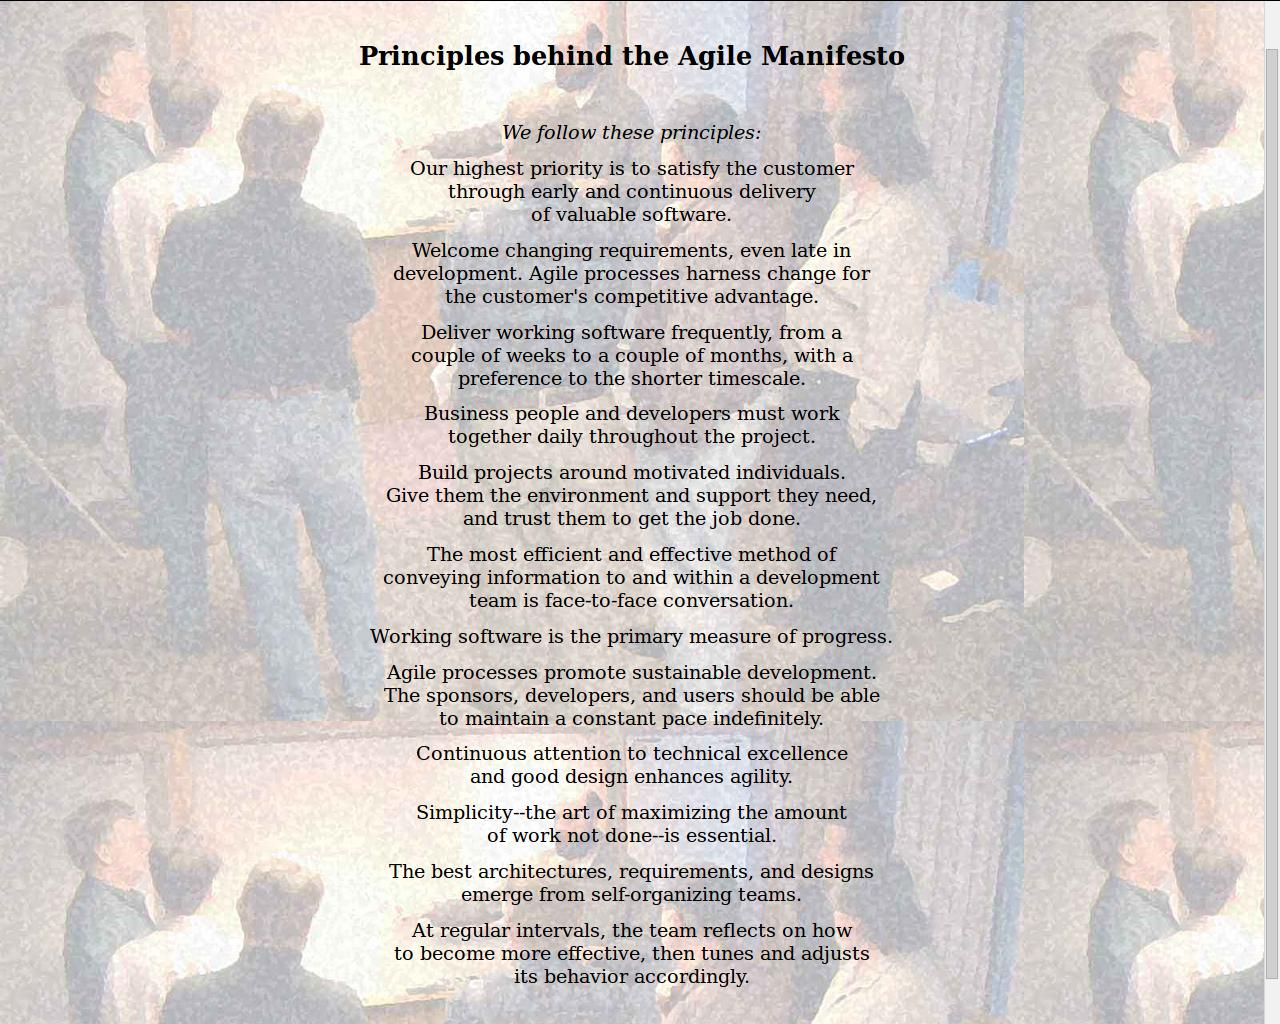
\includegraphics[width=0.7\textwidth]{fig/principios.jpg}
\end{center}
\caption{Principios del Manifiesto Ágil, en su web}
\label{fig:principios}
\hrule
\end{figure}

Estos principios marcan la diferencia entre los procesos tradicionales
y los considerados ágil. Los dos principios iniciales son genéricos a
todo el proceso, se consideran un resumen del estilo ágil.


\section{Programación Extrema}
\label{sec:xp}

La programación extrema (XP) es una de estas metodologías ágil que se
basa en los cuatro valores descritos en el apartado anterior y sigue
sus doce principios. En concreto esta metodología se diseña para
proyectos con requisitos muy imprecisos y cambiantes donde la relación
con el cliente y una buena comunicación en el equipo son esenciales.

El apellido \lst{extrema} se lo da Kent Beck, uno de los firmantes del
manifiesto ágil, porque coge los principios y los lleva al extremo en
la aplicación. Se asume que el proyecto va a tener muchos cambios y se
quiere reducir el coste de aplicarlos. Algunas de las características
son:
\begin{itemize}
\item Comunicación entre cliente y programadores de manera directa
  aunque supervisada. Siempre que se habla de la herramienta a
  desarrollar habrá al menos un experto miembro del equipo de
  desarrollo presente.
\item Se produce rápido por medio de entregas pequeñas. Se pone como
  máximo 3 meses para realizar una entrega. Aunque se recomienda no
  llegar a tanto.
\item La herramienta se describe mediante metáforas, ayudando a
  cliente y desarrolladores a hablar de lo mismo sin utilizar
  tecnicismos.
\item Se diseña siempre pensando en la simplicidad, se debe
  implementar la solución más sencilla que funcione.
\item Cada modificación realizada en el desarrollo debe superar una
  batería de pruebas unitarias establecidas con el cliente.
\item Trabajar en parejas es un requisito de modo que se reducen
  errores, se mejora el diseño, etc.
\item Se establece un máximo en el número de horas semanales, nadie
  podrá trabajar más de 40 horas a la semana.
\item El cliente debe tener disponibilidad constante para el equipo.
\item Programación mediante estándares, de modo que todo programador
  que coja el código sepa que ha hecho un programador anterior.
\end{itemize}
Estas prácticas junto con otras conforman la manera de trabajar
mediante una metodología XP. En Figura~\ref{fig:xp} podemos ver la
relación entre estas prácticas de modo que si tienen una flecha
significa que se refuerzan mutuamente.


\begin{figure}[h]
\hrule\smallskip
\begin{center}
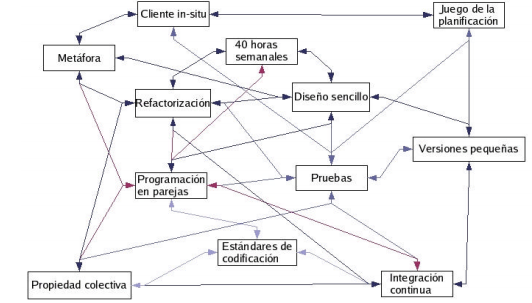
\includegraphics[width=0.9\textwidth]{fig/xp.png}
\end{center}
\caption{Relación de las características de XP}
\label{fig:xp}
\hrule
\end{figure}


Para llevar a cabo estas prácticas se utiliza una técnica conocida
como \emph{Historias de Usuario} donde se especifican los requisitos
mediante tarjetas de papel en las cuales el cliente describe
brevemente lo que un usuario debe poder hacer con la herramienta.

Kent Beck además define diferentes roles y dice que cada participante
en el proyecto debe tener uno de ellos:
\begin{itemize}
\item Programador
\item Cliente
\item Tester
\item Tracker
\item Entrenador
\item Consultor
\item Gestor
\end{itemize}

Las etapas del desarrollo quedan establecidas en 4, de manera cíclica:
\begin{enumerate}
\item El cliente define historias de usuario y su valor de negocio.
\item El programador estima el esfuerzo necesario para llevarlas a
  cabo.
\item El cliente decide qué se debe construir y sus prioridades,
  teniendo en cuenta las posibles restricciones de tiempo.
\item El programador implementa lo acordado.
\item Se vuelve al paso 1 hasta terminar el proyecto. Del 1 al 4 no
  deben pasar más de 3 meses.
\end{enumerate}

\section{Scrum}
\label{sec:scrum}

Scrum es una metodología ágil que se basa en la experiencia del equipo
y el conocimiento de los integrantes para realizar un desarrollo
fiable, de calidad y con producción incremental. Por eso se puede
decir que se caracteriza por:
\begin{itemize}
\item Adoptar una estrategia de desarrollo incremental, en lugar de la
  planificación y ejecución completa del producto.
\item Basar la calidad del resultado en el conocimiento tácito de las
  personas del equipo auto organizado.
\item Solapar las diferentes fase de desarrollo, en lugar de
  realizarlas de forma secuencial como ocurriría en otras metodologías
  más tradicionales.
\end{itemize}
Para llevar a cabo esta metodología se definen tres roles y divide el
tiempo en \lst{sprints}. Estos \lst{sprints} son la unidad básica de
medida y planificación. Se puede establecer la duración de un
\lst{sprint} en 10 días, aunque la duración puede variar en función de
la experiencia del equipo de desarrollo y de las tareas a
realizar. Suponiendo un \lst{sprint} de 10 días se sigue la siguiente
planificación:
\begin{itemize}
\item Día 1: Reunión de planificación del Sprint. Tiene una duración
  máxima de una hora. Se define que se desea hacer durante ese
  sprint. Se debe generar un acta o log con lo acordado.
\item Día 2-9: Reunión de Sprint. Tiene una duración máxima de 15
  minutos. Se realiza todos los días del sprint. No se realiza acta de
  la reunión. El ScrumMaster realiza a cada miembro del equipo las
  siguientes preguntas:
  \begin{itemize}
  \item ¿Qué hiciste ayer?
  \item ¿Qué harás para mañana?
  \item ¿Te ha surgido algún problema?
  \end{itemize}
\item Día 10: Reunión de Revisión del Sprint: Tiene una duración
  máxima de una hora. Se revisa el trabajo realizado y los objetivos
  alcanzados. Se puede mostrar demos del trabajo finalizado, pero
  nunca de partes parciales. Se genera un acta detallando los
  objetivos no alcanzados.  
\end{itemize}
Para garantizar la calidad de esta metodología basada en la calidad
del equipo de desarrollo se deben definir claramente unos roles que
garanticen el buen funcionamiento de la misma.
\begin{itemize}
\item \lst{Product Owner}: representa la voz del cliente. Se asegura
  de que se realicen las tareas adecuadamente desde una perspectiva de
  negocio.
\item \lst{Scrum Master (facilitador)}: trata de eliminar todos los
  obstáculos que impiden que el equipo alcance los objetivos del
  Sprint actual. No es el líder del equipo, el equipo es
  auto-organizado. El ScrumMaster asegura que el equipo no se
  distraiga del objetivo y cumpla las reglas de la metodología Scrum.
\item \lst{Desarrollador}: Realiza el producto con su equipo.
\end{itemize}

\chapter{Conclusiones}
\label{ch:conclusiones}

En este trabajo se han presentado dos metodologías ágiles que junto
con la expuesta por Dña. Simona se han extraído una serie de
características comunes y comparado con otras metodologías más
tradicionales. En el Cuadro~\ref{tabla:comparativa} se puede apreciar esta
comparativa a grandes rasgos.\\



\begin{table}[]
\centering
\caption{Comparativa entre metodologías ágiles y tradicionales.}
\label{tabla:comparativa}
\begin{tabular}{|p{7cm}  | p{7cm} |}


\hline
\textbf{Metodologías Ágiles} & \textbf{Metodologías Tradicionales} \\
\hline
Costumbres e ideas de desarrollo. & Normas de desarrollo. \\
\hline
El cambio es lo habitual. & Plan rígido, cambios costosos. \\
\hline
Autogestionada por el equipo. & Impuestas por una dirección \\
\hline
Poco control, basado en pocos principios. & 
Proceso muy controlado, con normas y procedimientos. \\
\hline
Contrato flexible. & Contrato detallado y fijo. \\
\hline
Cliente es parte del equipo. & Cliente interactúa mediante
reuniones. \\
\hline
Grupos pequeños(<10) y juntos. & Grupos grandes y distribuidos. \\
\hline
Pocos roles. & Más roles. \\
\hline

\end{tabular}

\end{table}

\section{Experiencia Personal}
\label{sec:experiencia}

En los últimos años vengo experimentando el uso de diferentes
metodologías para el desarrollo de proyectos. A continuación, se
realiza un repaso de algunos ``proyectos'', la metodología utilizada,
la sensación percibida por el equipo y sus resultados. \\


El primer proyecto llevado a cabo podría situarlo en 2011 en la
asignatura de Ingeniería del software. Desarrollamos entre 8 personas
una tienda virtual, siguiendo el modelo en espiral de Boehm. En este
proyecto sufrimos la inexperiencia del equipo y la carga repetitiva
que llevaba este modelo de trabajo, dado que cada vez que pasamos a
una fase debíamos repetir pasos ya realizados en la misma fase pero en
etapas anteriores. El producto final resultó de baja calidad pero con
gran documentación y la experiencia desastrosa, llegando al punto de
no querer volver a utilizar el modelo elegido.\\

Otro proyecto que puedo mencionar es en 2014 en la asignatura de
Desarrollo de Sistemas Informáticos. Utilizamos el modelo de
prototipos en un equipo formado por 4 personas. Se escogió esta
metodología porque el objetivo no era realizar una aplicación
funcional sino generar una buena interfaz para que los usuarios tengan
una buena experiencia utilizando la aplicación (un reproductor de
música). Las sensaciones recibidas fueron mucho mejores que con el
modelo en espiral, aunque es cierto, que el realizar solamente
prototipos nos resultó complicado, pues siempre intentábamos completar
las funcionalidades. Los resultados fueron algo satisfactorios
quedando la aplicación muy bien valorada por el resto de la clase.\\

El siguiente proyecto lo realicé en la empresa Coritel, consistía en
una serie de prototipos para una página web de hoteles. La metodología
utilizada era \emph{ágile} en ella se dio gran libertad a todos los
integrantes del equipo (4 personas en este caso) y se realizó de
manera incremental con revisiones quinquenales. La sensación fue en
gran parte de descontrol dado que era la primera toma de contacto con
una metodología no guiada paso a paso, pero los resultados fueron
prometedores y el cliente real quedó bastante satisfecho.\\

Los tres siguientes proyectos se han realizado en el ámbito del Máster
en Informática, en las asignaturas Dirección y Gestión de proyectos
informáticos, donde volvimos a una metodología de trabajo tradicional
guiada por el libro PMBOK, centrándonos en la dirección del
proyecto. La calidad de la documentación generada me sorprendió
gratamente y el proceso del proyecto resultó ser muy guiado y
evolutivo, pero la aplicación resultante dejó mucho que desear.\\

En las dos siguientes asignaturas se utilizó la metodología Scrum, en
la cual asumí el rol de \lst{Product Owner} y la de \lst{Scrum Master}
respectivamente a Tecnología Multimedia e interacción y la asignatura
Desarrollo de Aplicacione y Sistemas Inteligentes (DASI). Estos dos
proyectos (a mi parecer), han producido grandes resultados. De hecho,
en la asignatura de DASI, fuimos valorados como la mejor aplicación
por la mayoría de los compañeros. El proceso de revisión cada 10-15
días de Scrum y la poca carga documental, un acta y una matriz de
seguimiento de tareas, hicieron que los esfuerzos recayeran en la
aplicación sin descontrolar el crecimiento de la herramienta.\\

Por último, la participación en tres ediciones del concurso SWERC, en
dos del tuenti Contest, una code jam y más concursos de programación,
hicieron que aplicaramos técnicas de desarrollo sacadas de la
metodología de XP. Esto se debió a la necesidad de producir enseguida,
confiando en la experiencia del equipo donde es muy importante el test
de la aplicación, ya que fallar penaliza y un desarrollo temprano.\\

Estas y otras experiencias en el desarrollo de proyectos tanto a nivel
de estudiante como profesional me dejan bastante convencido de que es
bueno utilizar metodologías ágiles, confiando bastante en Scrum como
una metodología muy a tener en cuenta a la hora de realizar un
proyecto. Pero siempre teniendo en cuenta la naturaleza y finalidad
del proyecto, tal y como nos demuestra la Figura~\ref{fig:comic}. \\


\begin{figure}[h]
\hrule\smallskip
\begin{center}
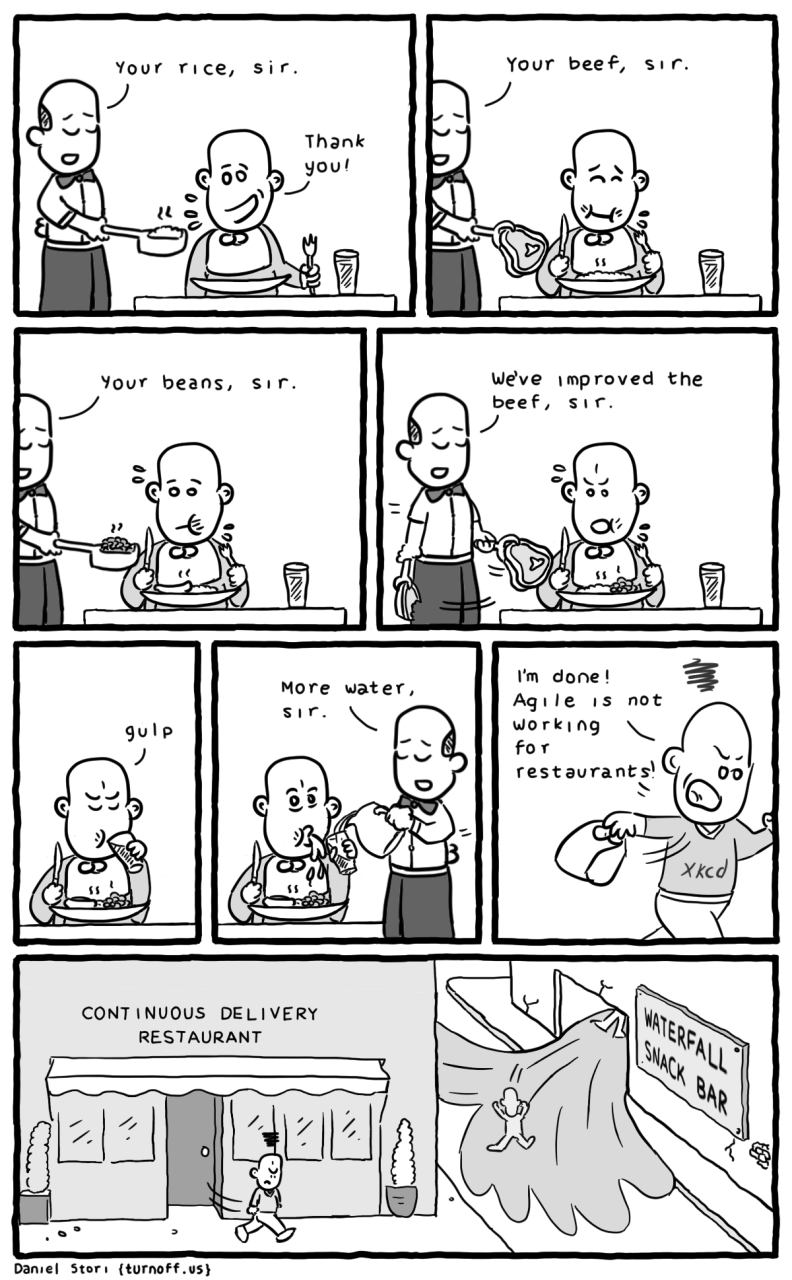
\includegraphics[width=0.9\textwidth]{fig/comic.jpg}
\end{center}
\caption{Usar metodologías ágiles no siempre es lo mejor}
\label{fig:comic}
\hrule
\end{figure}

\chapter{Bibliografía}
\label{biblio}

\begin{enumerate}
\item “IEEE Standard Glossary of Software Engineering Terminology,” IEEE std 610.12-1990, 1990. ISBN 155937067X.
\item SWEBOK executive editors, Alain Abran, James W. Moore; editors, Pierre Bourque, Robert Dupuis. (2004). Pierre Bourque and Robert Dupuis, ed. Guide to the Software Engineering Body of Knowledge - 2004 Version. IEEE Computer Society. pp. 1-1. ISBN 0-7695-2330-7.
\item R. Pressman: Ingeniería del Software - Un enfoque práctico, 7ª edición. McGraw - Hill, 2010.
\item Manifiesto Ágil, http://www.agilemanifesto.org/
\item I. Sommerville: Ingeniería del Software, 7ª edición. Addison Wesley, 2006
\item Henrik Kniberg: Scrum y XP desde las trincheras, borrador de traducción, 2007
\item "Manifesto for Agile Software Development", Agile Alliance, 2001
\item Southwestern Europe Regional Contest (SWERC), ACM
\item Felix y Steven Halim: Competitive Programming 3: The New Lower Bound of Programming Contests, 3ª Edición, 2013

\end{enumerate}



\end{document}

%%% Local Variables:
%%% mode: latex
%%% TeX-master: "manual"
%%% End:
